\documentclass[aspectratio=169, usepdftitle=false, xcolor={dvipsnames}, 9pt,table]{beamer}

\usetheme[english, notoc, coloraccent=blue]{awesome}

\title{Méthodes pour l'évaluation de l'activité cyclonique tropicale en changement climatique}
\author[William]{William Dulac}
\subtitle{Soutenance de thèse}
\email{william.dulac@meteo.fr}
\institute{Centre National de Recherches Météorologiques}
\uni{Université Paul Sabatier -- Toulouse III} 
\location{Toulouse}
\date{20 Décembre 2023}

\supervisors{Julien Cattiaux, Fabrice Chauvin}
\reporters{Jean-Philippe Duvel, Sylvie Malardel}
\examinators{Jean-Pierre Chaboureau, Christophe Menkes,\par\hspace*{16ex}Caroline Muller}

\background{include/Bolaven_2023-10-11_2300Z.jpg}

\usefonttheme[onlymath]{serif}

%\setlength\abovecaptionskip{-1pt}

\addbibresource{references.bib}

\newcommand\blfootnote[1]{%
  \begingroup
  \renewcommand\thefootnote{}\footnote{#1}%
  \addtocounter{footnote}{-1}%
  \endgroup
}

\begin{document}

\maketitle

\section[Introduction]{Introduction : Cyclones tropicaux}

\makesecslide

\subsection{Définition}

%===================================================
\begin{frame}[t]
    \renewcommand*{\thefootnote}{\fnsymbol{footnote}}
    \frametitle{Qu'est-ce qu'un cyclone tropical (TC) ?}
    \framesubtitle{Définition et ordres de grandeur}

    \begin{center}
        \begin{minipage}{0.7\linewidth}
            \begin{definition}
                \footnotesize
                \centering
                Larges systèmes dépressionnaires et tourbillonnaires se développant sur océan dans les tropiques et caractérisés notamment par la présence d'un
            \textquote{œil} en leur centres
            \end{definition}
        \end{minipage}
    \end{center}
    %
    \begin{columns}
        \begin{column}{0.5\textwidth}
            \begin{figure}[h]
                \centering
                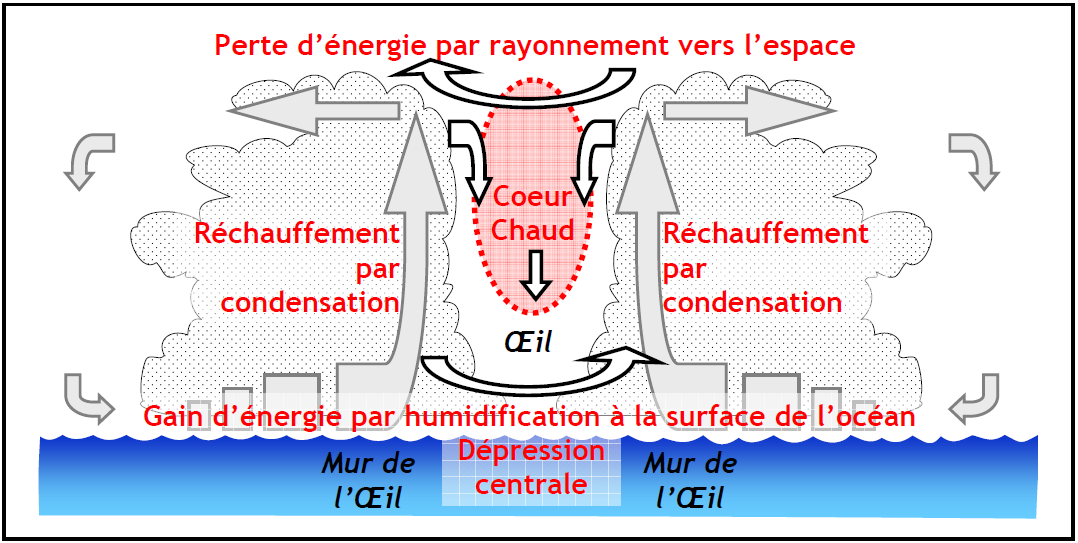
\includegraphics[width=\textwidth]{Figures/cyclones1_fig3_Cycle-thermodynamique-cyclone.png}
                \caption{Cycle thermodynamique d'un cyclone tropical à maturité\\
                \textit{Illustration de Frank Roux pour l'Encylopédie de l'Environnement, 20 Septembre 2018}}
            \end{figure}
        \end{column}
        \begin{column}{0.5\textwidth}
           \setlength{\leftmargini}{2.5ex}
           \vspace{-2em}
           \begin{block}[Grandeurs caractéristiques] 
                \footnotesize
                \begin{itemize}
                    \item Fréquence annuelle moyenne : 84 TC par an \mbox{\parencite{schreck_impact_2014}}
                    \item Diamètre moyen de l'œil : 55 \sim~85 km \mbox{\parencite{weatherford_typhoon_1985}}
                    \item Diamètre\footnotemark~total moyen: 500 km \parencite{carrasco_influence_2014}
                    \item Vitesse de déplacement moyenne : 20 km/h
                    \item Vents soutenus : Entre 120 et 300 km/h
                \end{itemize}
            \end{block}
        \end{column}
    \end{columns}
    \footnotetext{Basé sur la mesure ROCI (\textit{Radius of Outermost Closed Isobar})}
    \renewcommand*{\thefootnote}{\arabic{footnote}}
    \setcounter{footnote}{0}
\end{frame}

%===================================================
\begin{frame}[c]
    \frametitle{Qu'est-ce qu'un cyclone tropical ?}
    \framesubtitle{Bassins d'activité et classification}
    \begin{columns}
        \begin{column}{0.65\textwidth}
            \begin{figure}[h]
                \centering
                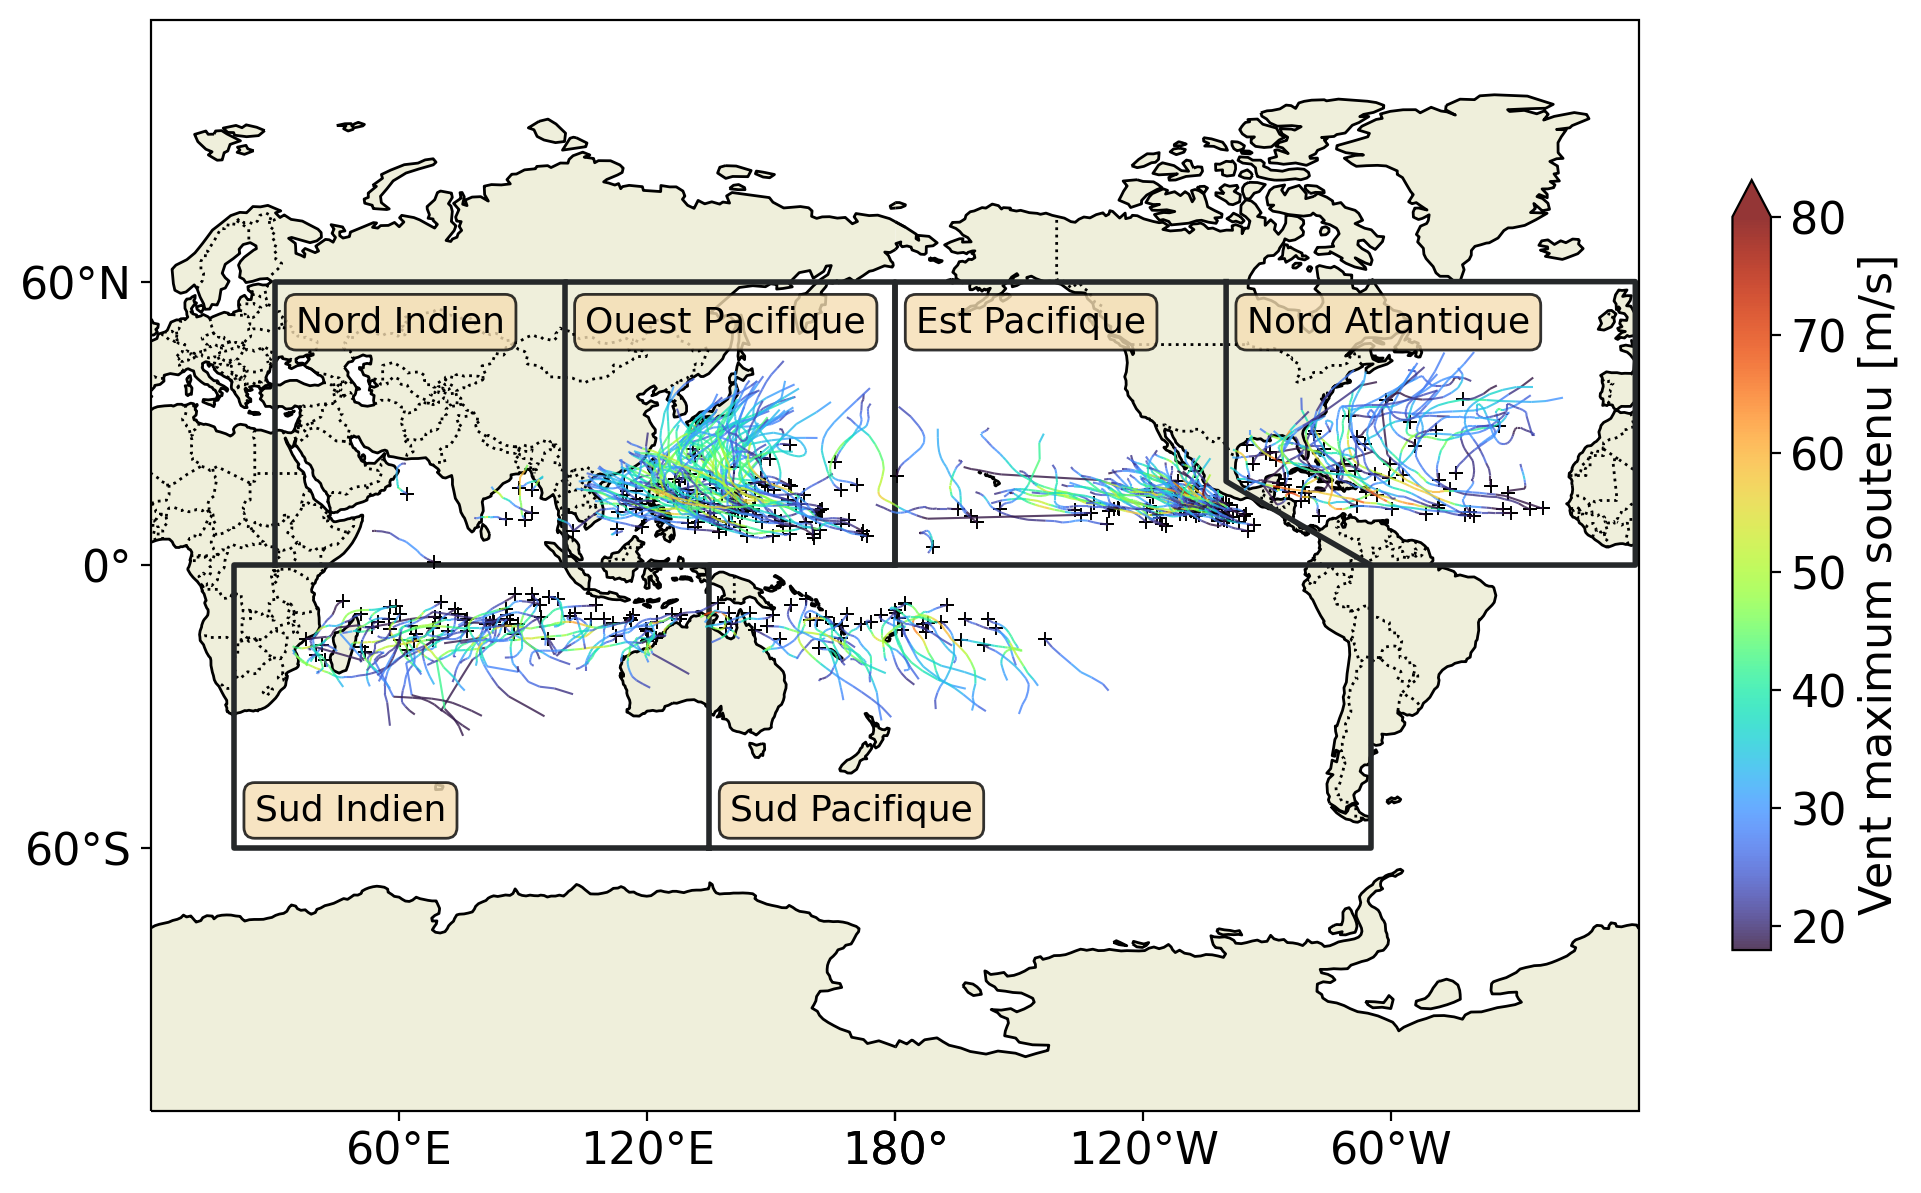
\includegraphics[width=\textwidth]{Figures/Bassins_et_trajectoires_soutenance.png}
                \caption{Échantillon de trajectoires historiques observées (IBTrACS) entre 1980 et 2019.}
            \end{figure}
        \end{column}
        \begin{column}{0.35\textwidth}
            \begin{table}[h]
                \centering
                \caption{Seuils de vents (sur 10 minutes) des catégories Saffir-Simpson (gauche) et seuils de pression équivalents ajustés
                selon \cite{klotzbach_surface_2020}.}
                \footnotesize
                \begin{tabular}{l|c|c}
                     & Vent (m/s) & Pression (hPa) \\
                    \hline
                    TD & $<$ 16 & $>$ 1005 \\
                    TS & 16 -- 28 & 1005 -- 991 \\
                    Cat 1 & 29 -- 37 & 990 -- 976 \\
                    Cat 2 & 38 -- 43 & 975 -- 961 \\
                    Cat 3 & 44 -- 51 & 960 -- 946 \\
                    Cat 4 & 52 --  62 & 945 -- 926\\
                    Cat 5 & $\geq$ 63 & $\leq$ 925
                \end{tabular}
            \end{table}
        \end{column}
    \end{columns}
\end{frame}

%===================================================
\begin{frame}[c]
    \frametitle{Qu'est-ce qu'un cyclone tropical ?}
    \framesubtitle{Conditions de formations}
    \begin{figure}[h]
        \centering
        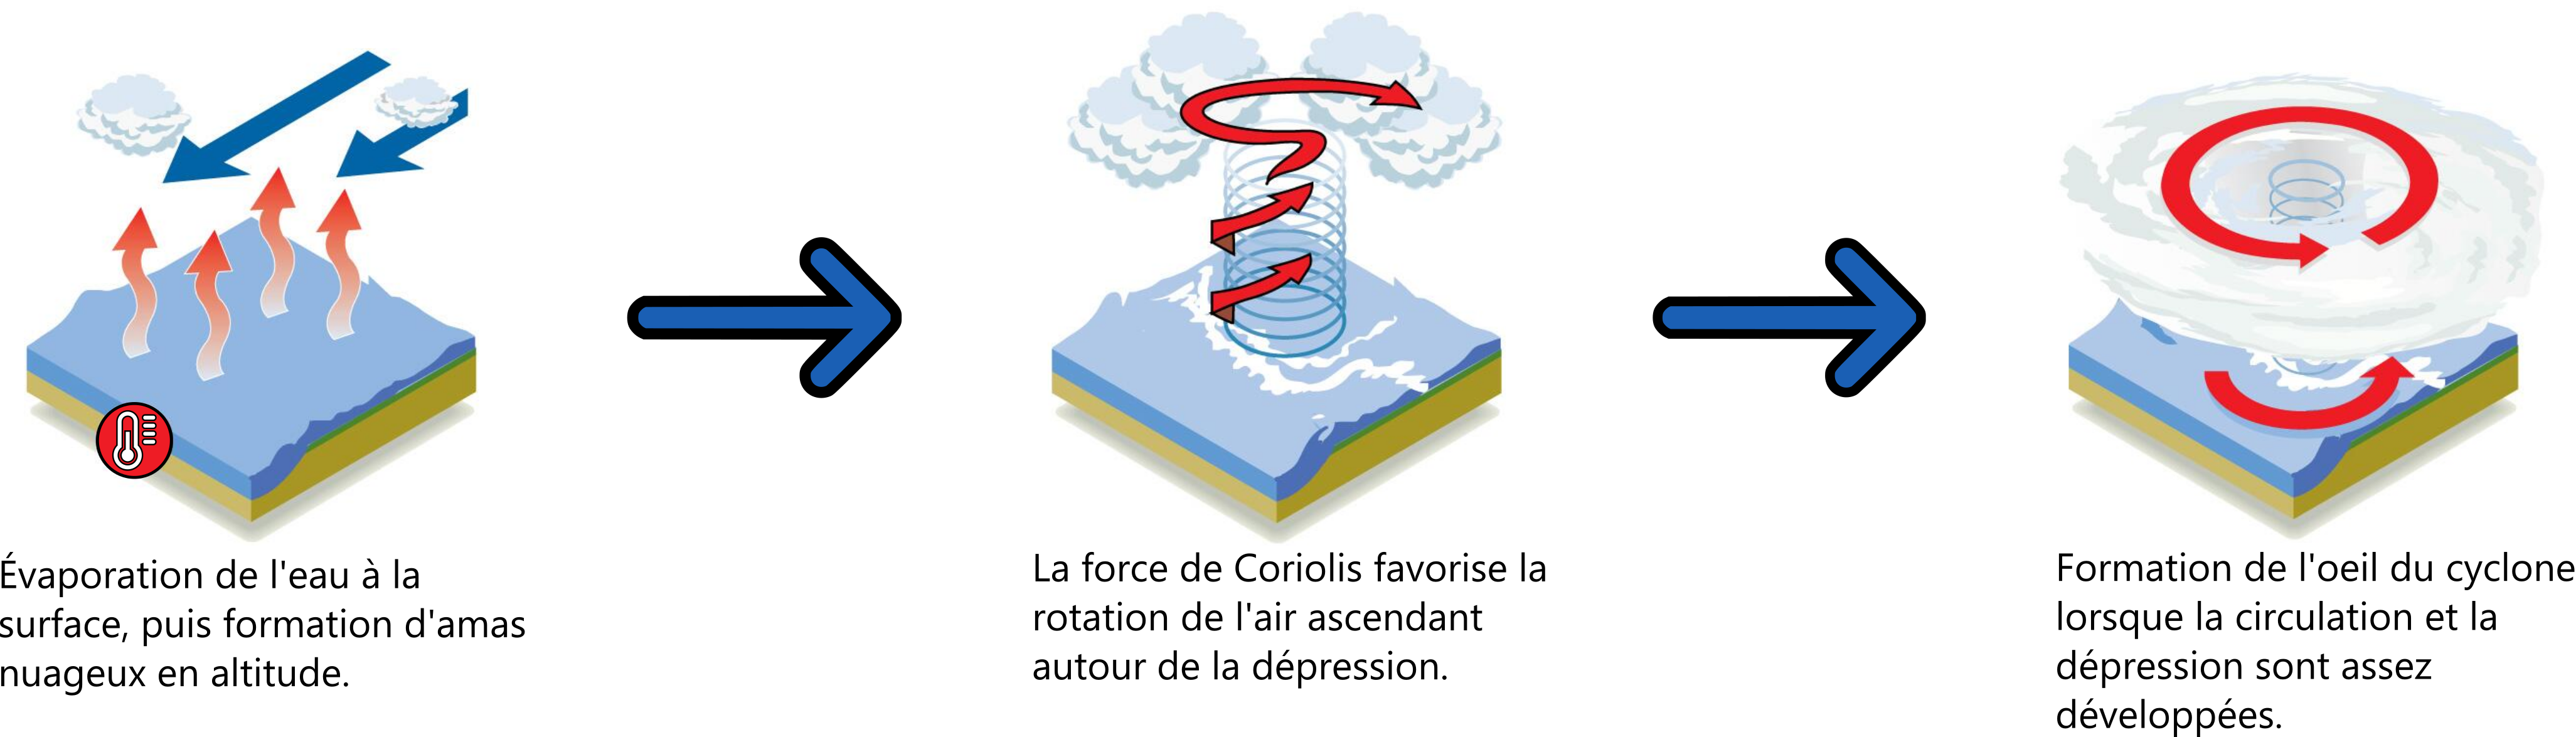
\includegraphics[width=0.8\textwidth]{Figures/diagramme_formation.png}
    \end{figure}
    %\vspace{1em}
    \footnotesize
    \begin{block}[Ingrédients de la cyclogénèse]
        \begin{columns}[t]
            \scriptsize
            \begin{column}{0.5\textwidth}
                \begin{itemize}
                   \item Perturbation initale apportant de la convergence en basses couches
                   \item Une distance de quelques centaines de kilomètres à l'équateur (Coriolis)
                   \item Température de surface de l'ocean supérieure à 26°C sur au moins 60m de profondeur \parencite{palmen_formation_1948}
                \end{itemize}
            \end{column}
            \begin{column}{0.5\textwidth}
               \begin{itemize}
                   %\setlength{\leftmargini}{1.5ex}
                   \item Absence de cisaillement vertical du vent\\\parencite{gray_global_1968}
                   \item Atmosphère humide en moyenne troposphère
                   \item Atmosphère instable
               \end{itemize} 
            \end{column}
        \end{columns}
    \end{block}
    \blfootnote{Illustration adaptée d'une infographie AFP existante}
\end{frame}

%===================================================
\begin{frame}[c]
    \frametitle{Qu'est-ce qu'un cyclone tropical ?}
    \framesubtitle{Le phénomène météorologique le plus destructeur}
    \begin{definition}
        \footnotesize
        \begin{itemize}
            \item Plus de 400 000 morts et près de 300 000 blessés entre 1980 et 2009 \parencite{doocy_human_2013}.
            \item 20 millions de personnes rendues sans-abri \parencite{doocy_human_2013}.
            \item Coût économique moyen de plus de 20 milliards de dollars par cyclone (TC) aux États-Unis \parencite{smith_billiondollar_2020}.
        \end{itemize} 
    \end{definition}
    \begin{columns}
        \begin{column}{0.45\textwidth}
            \begin{figure}[h]
                \centering
                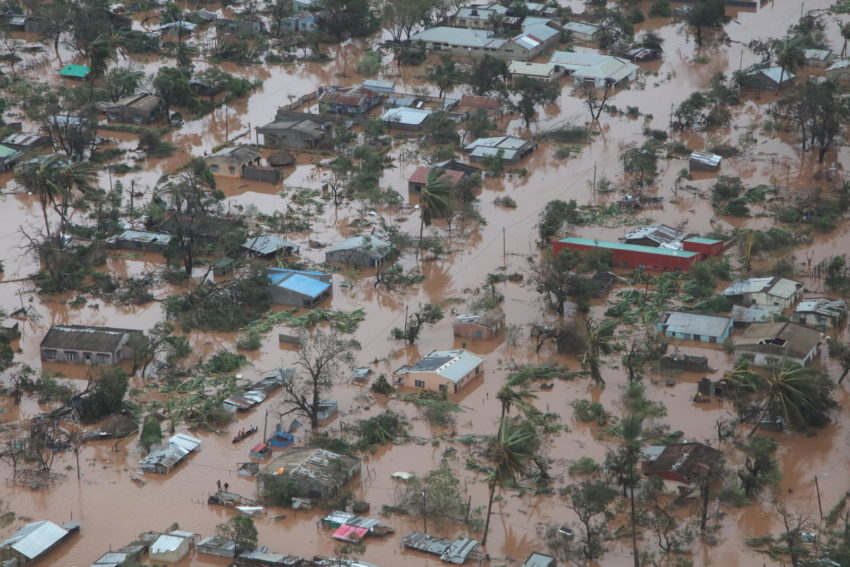
\includegraphics[width=0.97\textwidth]{Figures/idai_2019_sofala_province.jpg}
                \caption{Povince de Sofala au Mozambique après le passage du \mbox{cyclone} Idai, Mars 2019. \textit{Photo de l'Institut National
                de Gestion des Catastrophes du Mozambique (INGC).}}
            \end{figure}
        \end{column}
        \begin{column}{0.45\textwidth}
             \begin{figure}[h]
                 \centering
                 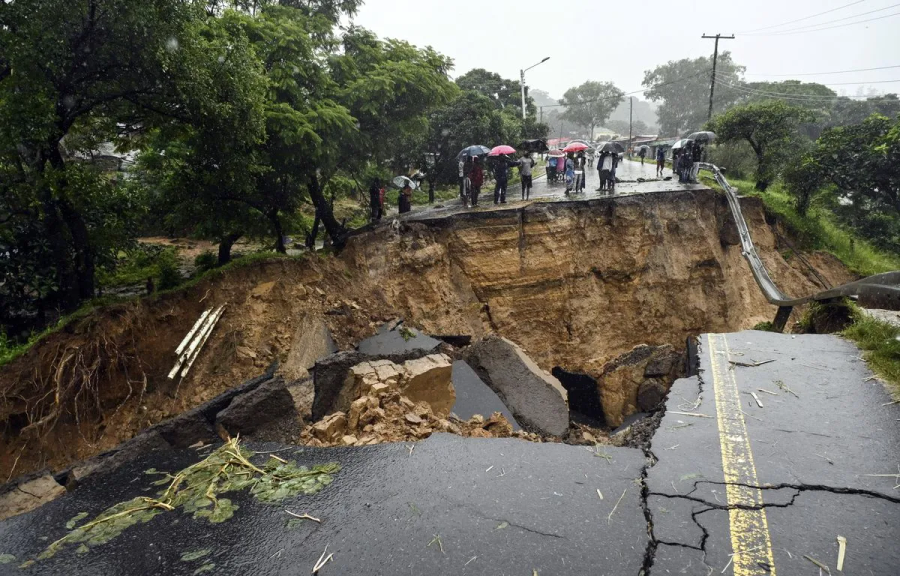
\includegraphics[width=\textwidth]{Figures/freddy_malawi_route.png}
                 \caption{Route endommagée au Malawi après le passage du cyclone Freddy, Mars 2023.\\\textit{Photo AP/SIPA/Thoko Chikondi}}
             \end{figure}
        \end{column}
    \end{columns}
\end{frame}

\subsection{Consensus sur les projections futures}

%=========================================================
\begin{frame}[c]
    \frametitle{Consensus sur l'évolution future de l'activité cyclonique}
    \begin{columns}
        \begin{column}{0.75\textwidth}
            \begin{figure}
                \centering
                \begin{tikzpicture}
                    \node[anchor=south west, inner sep=0] (image) at (0,0)%
                        {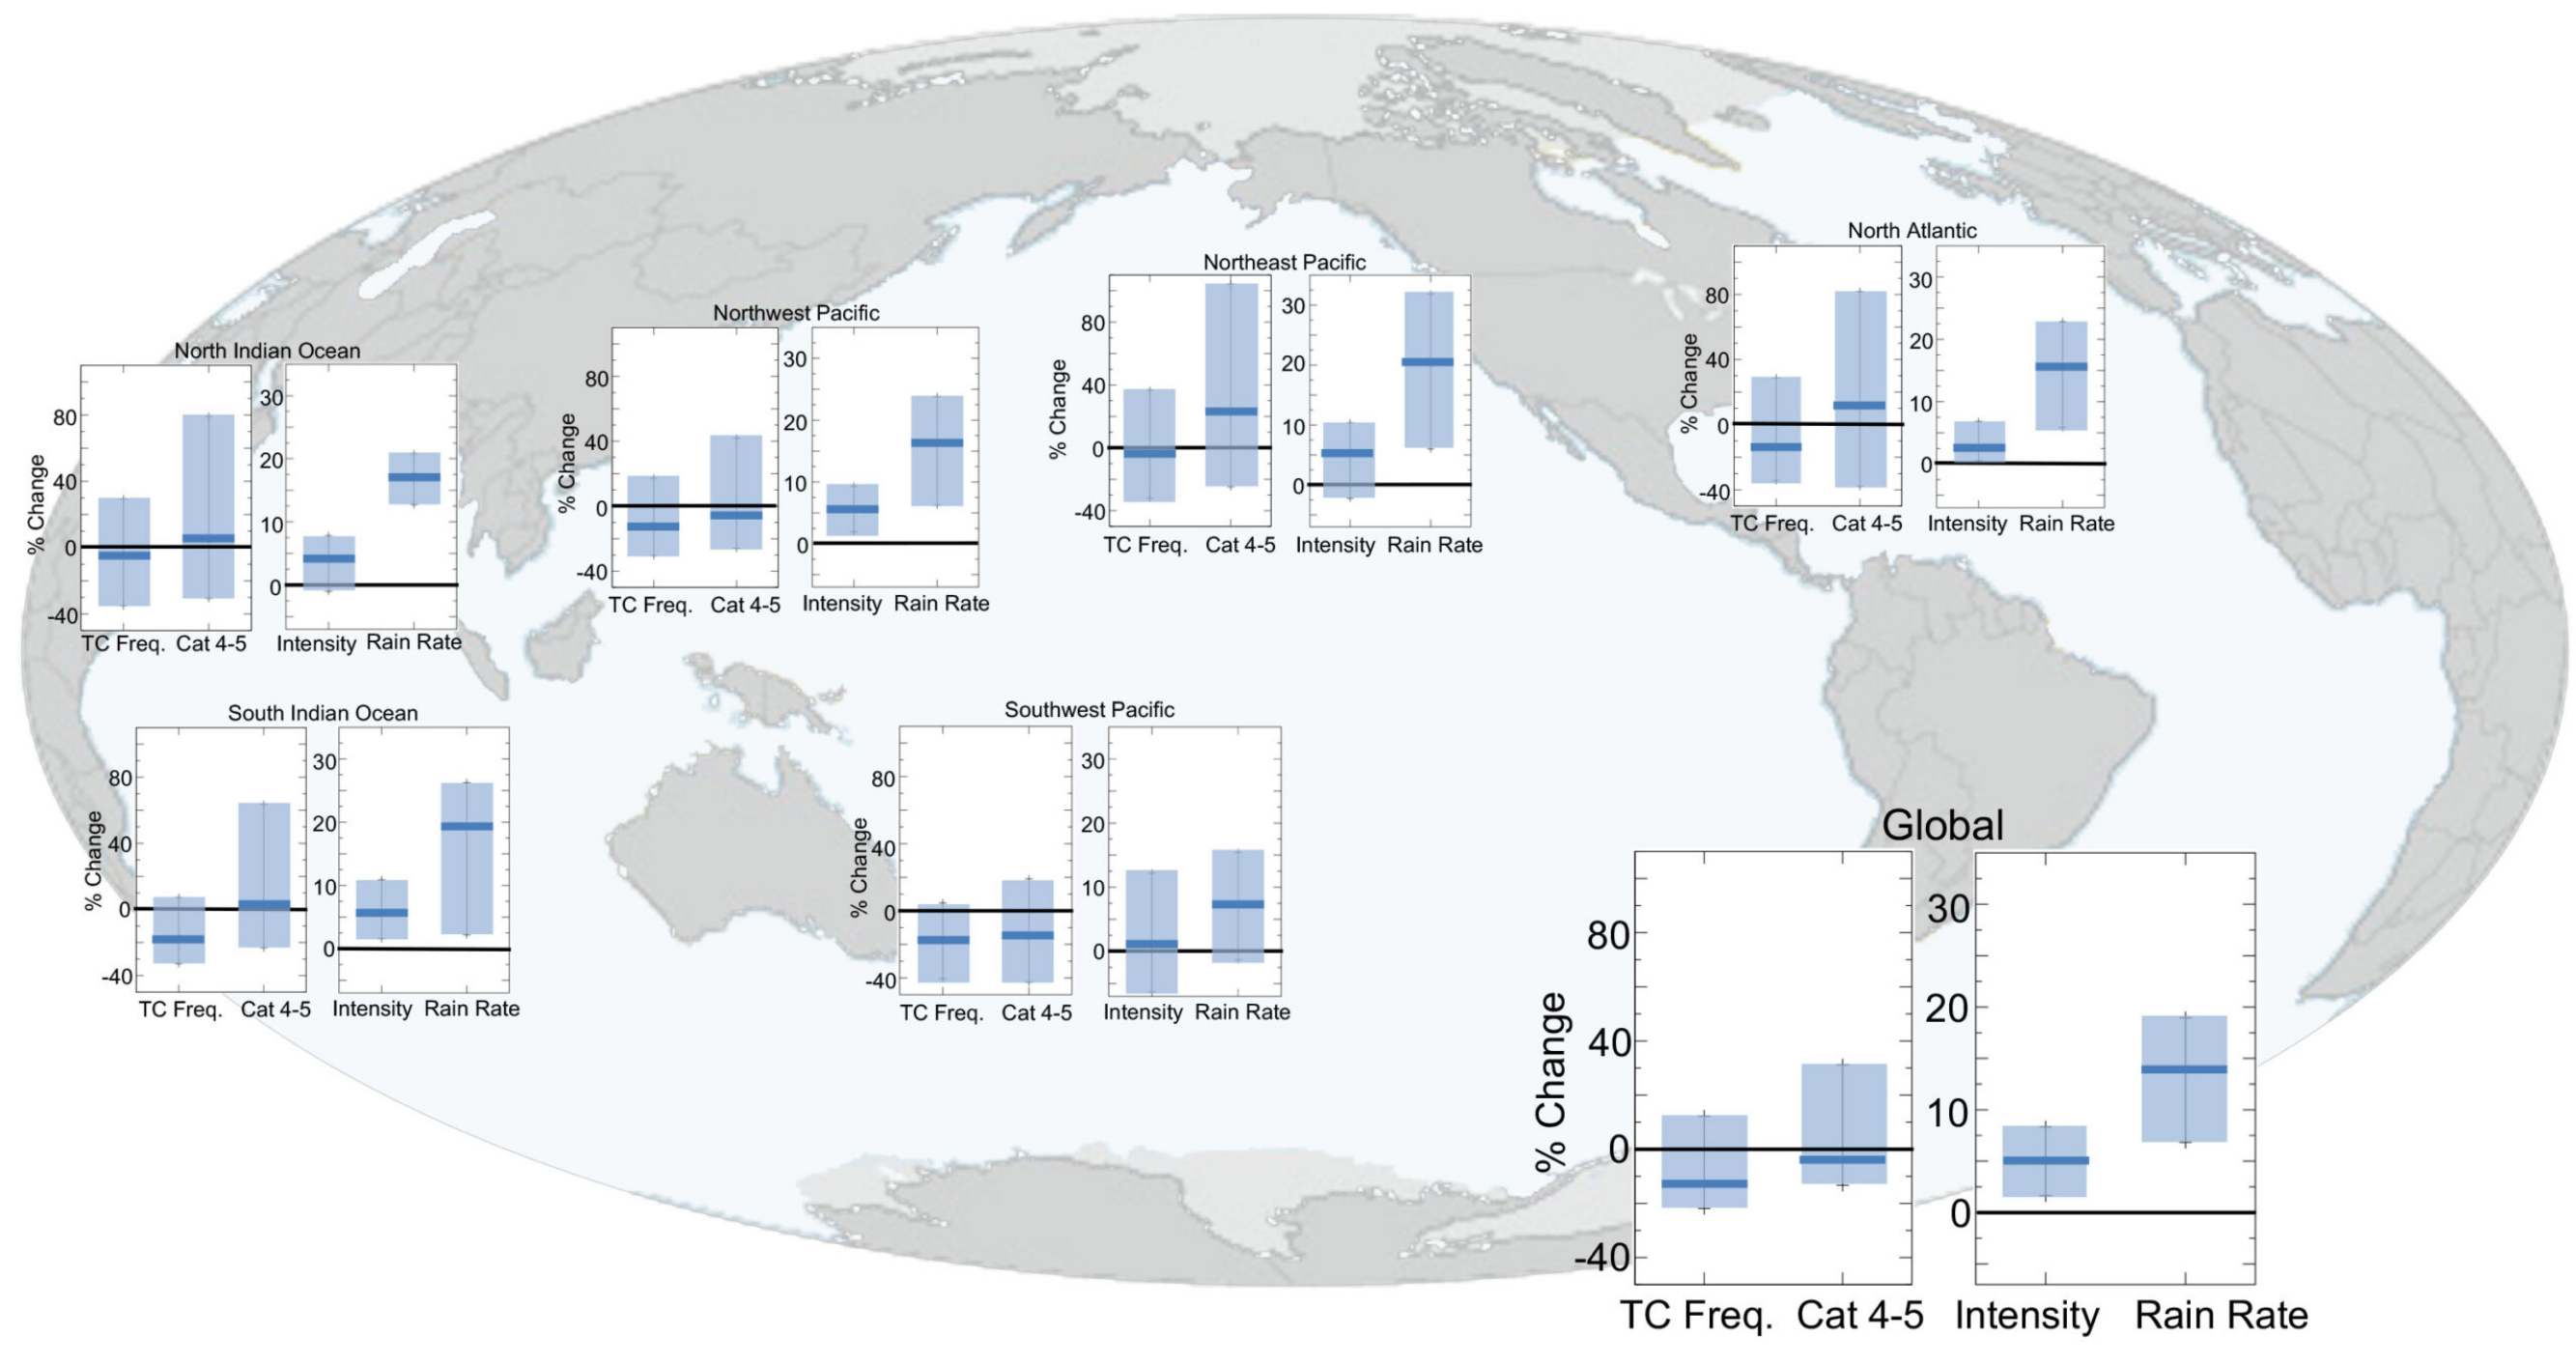
\includegraphics[width=\textwidth]{Figures/Fig_5_Knutson_BAMS_revised_3_9_20-scaled_cropped.png}};
                    \begin{scope}[x={(image.south east)},y={(image.north west)}]
                        \draw[rounded corners=0.5mm, red, fill, fill opacity=0.1, line width=0.5] (0.627, 0.018) rectangle (0.69, 0.055);
                        \draw[rounded corners=0.5mm, green, fill, fill opacity=0.1, line width=0.5] (0.6955, 0.018) rectangle (0.749, 0.055);
                        \draw[rounded corners=0.5mm, blue, fill, fill opacity=0.1, line width=0.5] (0.755, 0.018) rectangle (0.818, 0.055);
                        \draw[rounded corners=0.5mm, purple, fill, fill opacity=0.1, line width=0.5] (0.825, 0.018) rectangle (0.898, 0.055);
                    \end{scope}
                \end{tikzpicture}
                \caption{Synthèse des projections de l'activité cyclonique pour un réchauffement de 2°C par rapport à 1986 -- 2005
                \parencite{knutson_tropical_2020}. Médianes et intervalles de confiance de respectivement 90~\% et 80~\% (gauche et droite).}
            \end{figure}
        \end{column}
        \begin{column}{0.25\textwidth}
           \footnotesize
           \setlength{\leftmargini}{2.5ex}
           \begin{block}[Résumé]
               \scriptsize
               \begin{itemize}
                    \item \textcolor{red}{Baisse} probable de la fréquence en général 
                    \item \textcolor{green}{Hausse} \underline{relative} de la fréquence des cyclones forts
                    \item \textcolor{blue}{Hausse} fortement probable de l'intensité maximale
                    \item \textcolor{purple}{Hausse} très fortement probable des précipitations
               \end{itemize}
           \end{block}
           \pause
           \begin{alertblock}
                \scriptsize
                Incertitudes conséquentes, y compris parfois sur le signe du changement
           \end{alertblock}
        \end{column}
    \end{columns}
\end{frame}

\subsection[Méthodologies d'évaluation]{Comment sont réalisées ces projections ?}
\makesubsecslide

%=========================================================
\begin{frame}[c]
    \frametitle{Les modèles de climat}
    \framesubtitle{Simulation numérique de l'évolution de l'état de l'atmosphère}
    \begin{columns}
        \begin{column}{0.55\textwidth}
            \footnotesize
            \begin{definition} 
                Discrétisation de l'évolution de l'état de l'atmosphère dans le temps et \alert{l'espace}\\
                $\longrightarrow$ ~L'échelle de la \alert{maille}
            \end{definition}
            \vspace{1em}%
            \begin{block}[Résolutions horizontales des modèles actuels \parencite{ipcc_annex_2021}]
                \begin{itemize}
                    \item Hautes résolutions : 20 \sim~80 km
                    \item Basses résolutions : 100 \sim~250 km
                \end{itemize}
            \end{block}
            \vspace{1em}%
            \onslide<2->{
                \begin{alertblock}
                    On commence tout juste à pouvoir descendre à l'échelle nécessaire pour simuler des TC \underline{réalistes}
                \end{alertblock}
            }
        \end{column}
        \onslide<1->{
            \begin{column}{0.45\textwidth}
                \begin{figure}[t]
                    \centering
                    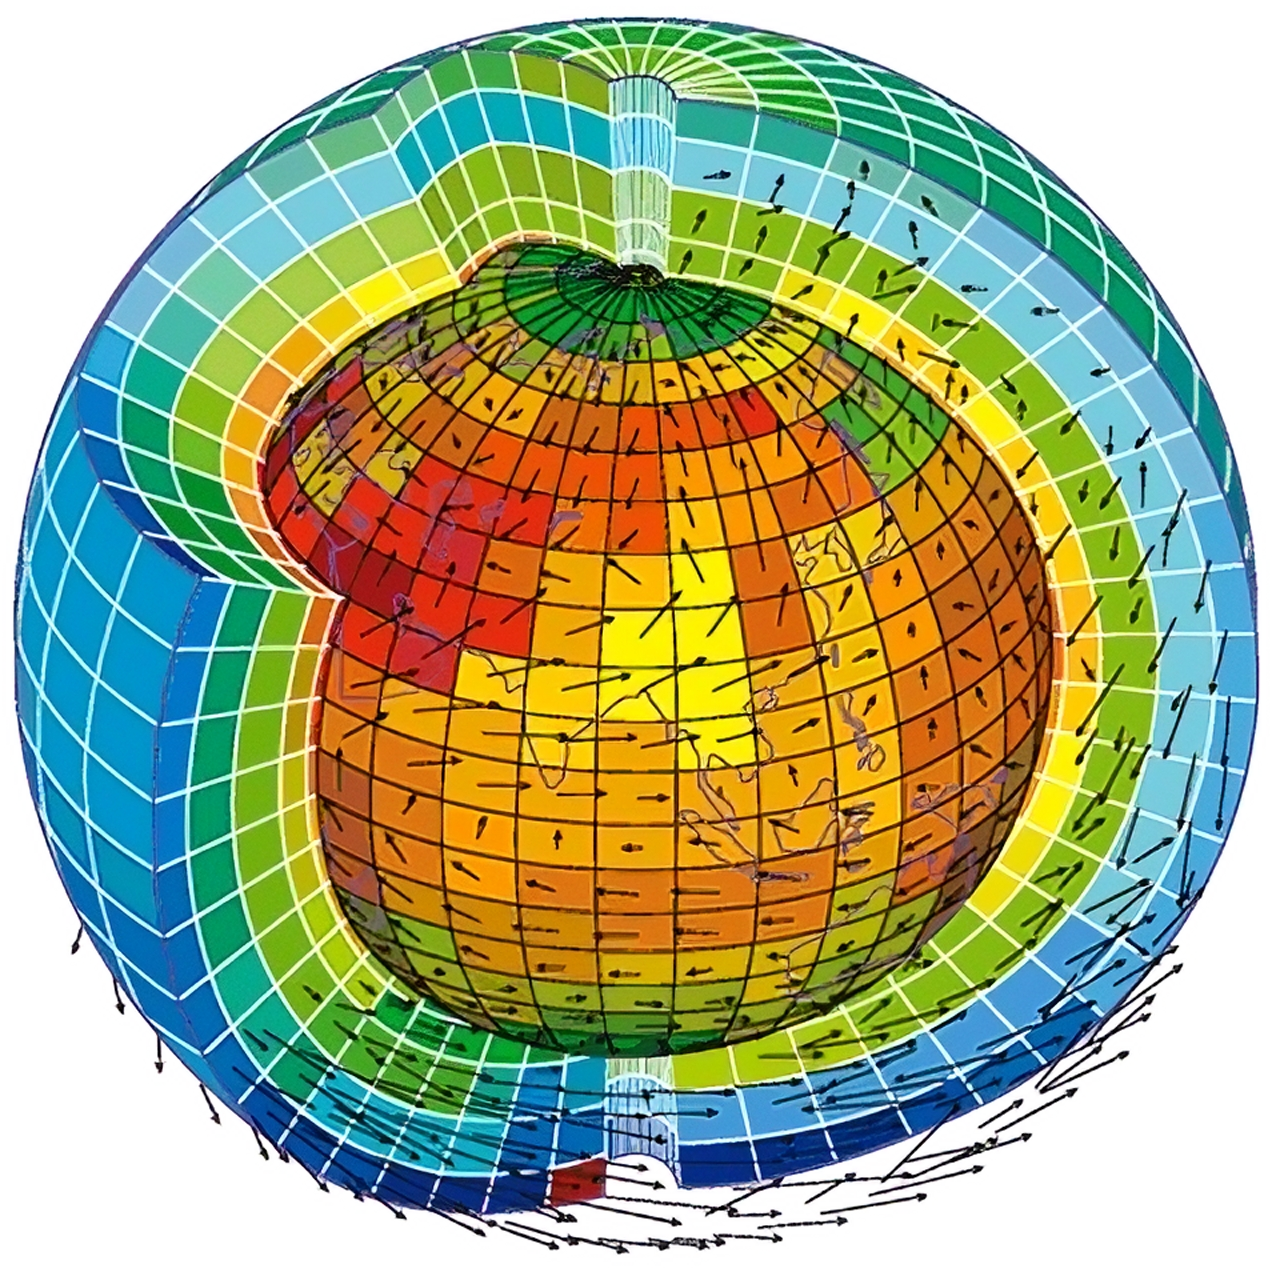
\includegraphics[width=0.8\textwidth]{Figures/maillage_upscaled_x4_2.png}
                    \captionsetup{width=0.9\textwidth}
                    \caption{Illustration schématique du maillage tridimensionnelle d'un modèle de climat. Les couleurs représentent la température et les flèches
                    le vent.\\\textit{Illustration de \mbox{Laurent Fairhead/LMD/CNRS}}.}
                \end{figure}
            \end{column}
        }
    \end{columns} 
\end{frame}

%=========================================================
\begin{frame}[c]
    \frametitle{Détection et suivi objectif}
    \framesubtitle{Mesure directe dans les simulations haute résolution}
    \begin{columns}
        \begin{column}{0.66\textwidth}
            \footnotesize
            \begin{definition}
                \centering
                Algorithmes identifiant et reliant entre eux les points de grille qui satisfont une ou plusieurs conditions.
            \end{definition}
            \vspace{1em}
            \onslide<2->{
                \begin{block}
                    \centering
                    Statistiques descriptives sur le nombre et les propriétés des cyclones détectées dans des simulations en climat futur
                \end{block}
            }
            \begin{columns}[t]
                \setlength{\leftmargini}{2.5ex}
                \begin{column}{0.45\textwidth}
                    \onslide<3->{
                        \begin{examples}[Intérêt principal]
                            \scriptsize
                            Mesure \alert{directe}
                            \tcblower
                            \scriptsize
                            \begin{itemize}
                                \item Capture le cycle de vie
                                \item Permet une évaluation de tous les aspects de l'activité cyclonique
                            \end{itemize}
                        \end{examples}
                    }
                \end{column}
                \begin{column}{0.45\textwidth}
                    \onslide<4->{
                        \begin{alertblock}[Inconvénients] 
                            \scriptsize
                            \begin{itemize}
                                \item Nécessite des simulations à haute résolution (coûteuses et encore trop peu nombreuses)
                                \item Sensibilité à la méthodologie de détection \parencite{horn_tracking_2014,bourdin_intercomparison_2022}
                            \end{itemize}
                        \end{alertblock}
                    }
                \end{column}
            \end{columns}
            %\vspace{1em}
        \end{column}
        %
        \onslide<1->{
                \begin{column}{0.33\textwidth}
                \captionsetup{width=4cm}
                \vspace{-3em}
                \begin{figure}
                    \centering 
                    \animategraphics[autoplay,loop,width=4cm,poster=22]{5}{Figures/Ophelia/vo850/ophelia-vo850-}{0}{27}
                    \caption{Animation du cyclone \href{run:./ophelia-vo850.gif}{Ophelia} (2017) sur fond de \alert{vorticité relative à 850 hPa} (ERA5)}
                \end{figure}
                %
                \begin{figure}
                    \centering
                    \animategraphics[autoplay,loop,width=4cm,poster=22]{5}{Figures/Ophelia/msl/ophelia-msl-}{0}{27}
                    \caption{Animation du cyclone \href{run:./ophelia-msl.gif}{Ophelia} (2017) sur fond de \alert{pression au niveau de la mer} (ERA5)}
                \end{figure}
            \end{column}
        }
    \end{columns}
\end{frame}

%=========================================================
\begin{frame}[t]
    \frametitle{Indices de cyclogénèse}
    \framesubtitle{Inférence de l'activité par l'environnement de grande échelle}
    \begin{columns}[t]
        \begin{column}{0.5\textwidth}
            \begin{definition}
                \scriptsize
                %\centering
                \underline{Fréquence d'occurrence} des TC en un point de grille proportionnelle à une \mbox{combinaison} de variables \alert{thermiques} et
                \mbox{\alert{dymamiques}} de grande échelle \parencite{gray_tropical_1975}.
            \end{definition}
            \onslide<2->{
                \vspace{1em}
                \begin{block}
                    \scriptsize
                    \centering
                    Relations établies en climat présent pour application à des simulations en climat futur.
                \end{block}
            }
            \begin{columns}[t]
                \setlength{\leftmargini}{2ex}
                \begin{column}{0.5\textwidth}
                    \onslide<3->{
                        \footnotesize
                        \begin{examples}[Intérêt principal]
                            \scriptsize
                            Applicable à des modèles basse résolution\\(plus nombreux \Rightarrow Meilleure estimation de l'incertitude)
                        \end{examples}
                    }
                \end{column}
                \begin{column}{0.5\textwidth}
                    \onslide<4->{
                        \footnotesize
                        \begin{alertblock}[Inconvénients]
                            \scriptsize
                            \begin{itemize}
                                \item Mesure \alert{indirecte}
                                \item Incertitudes sur le choix des variables
                            \end{itemize}
                        \end{alertblock}
                    }
                \end{column}
            \end{columns}
        \end{column}
        \begin{column}{0.5\textwidth}
            \vspace{-3em}
            \begin{figure}
                \centering
                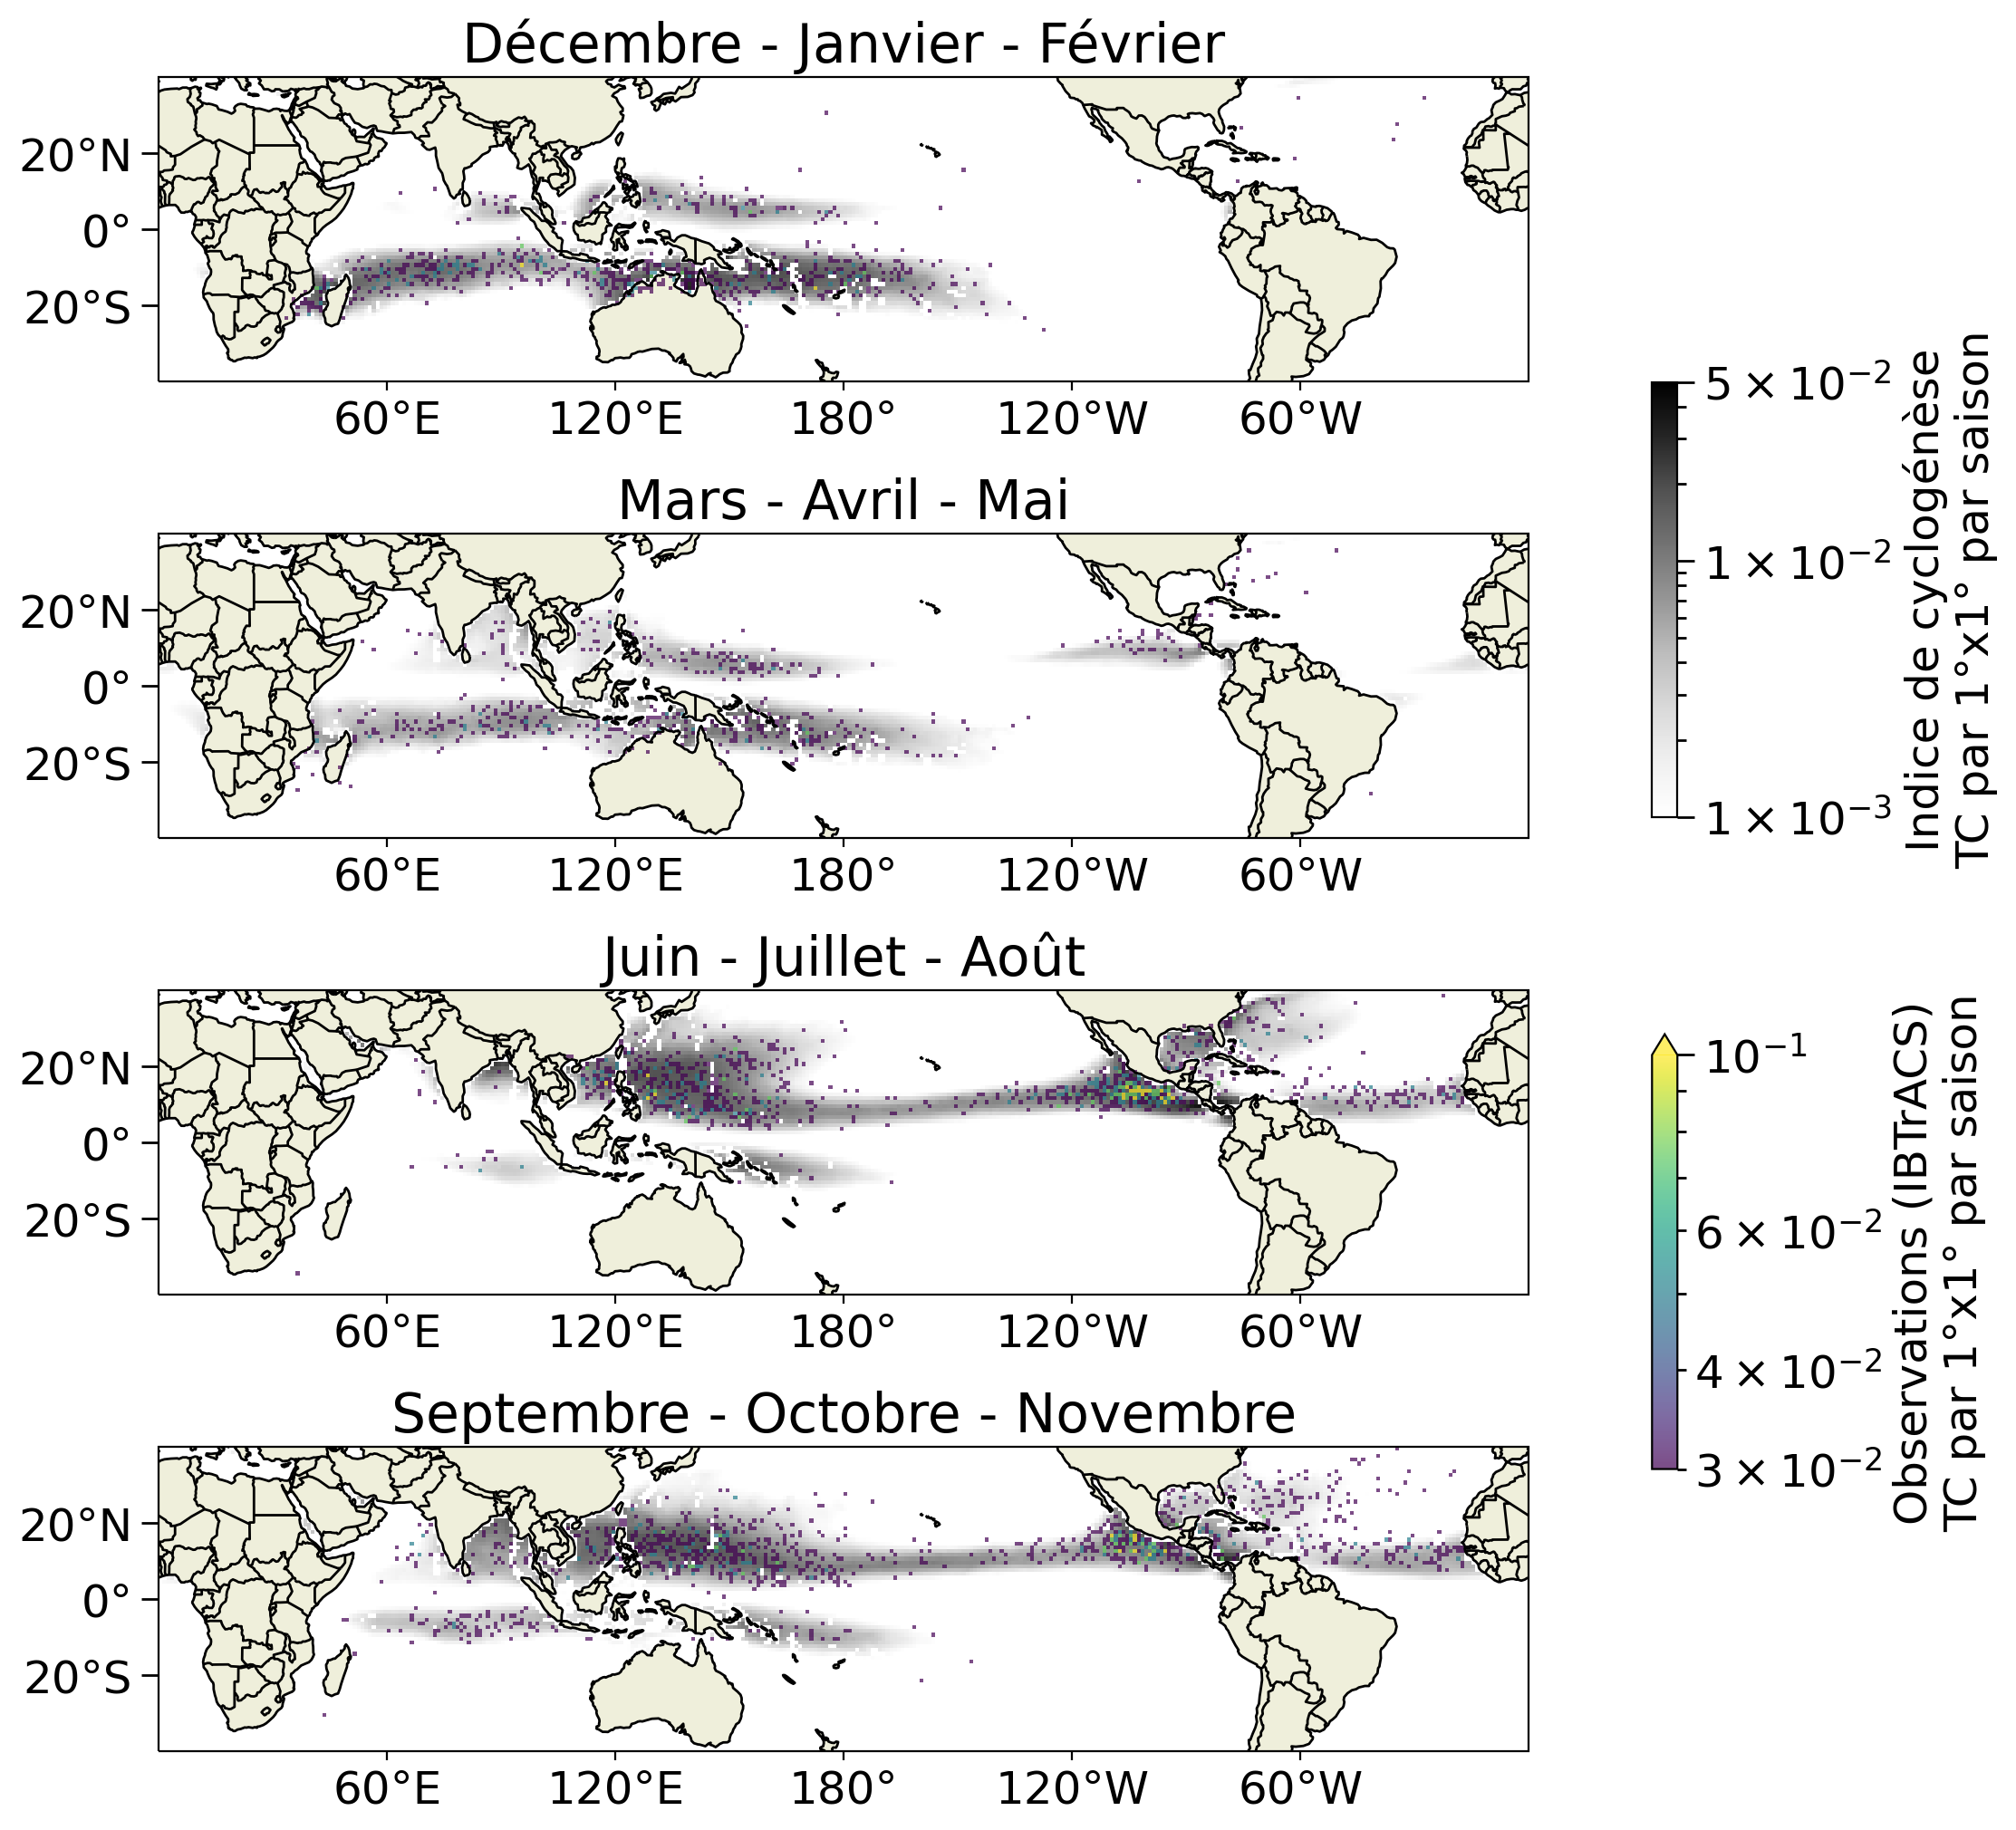
\includegraphics[width=\textwidth]{Figures/acgi_mean_IBTrACS_season.png}
                \caption{Moyennes saisonnières de trois indices moyennés entre eux (GPI, TCS et CYGP), et densité observée de cyclogénèse entre 1980 et 2019
                (IBTrACS).}
            \end{figure}        
        \end{column}
    \end{columns}
\end{frame}

%\begin{frame}[c]
%    \frametitle{Détection et suivi objectif}
%    \framesubtitle{Mesure directe dans les simulations}
%    %
%    \footnotesize
%    \begin{definition}
%        \centering
%        Algorithmes identifiant et reliant entre eux les points de grille qui satisfont une ou plusieurs conditions.
%    \end{definition}
%    \begin{columns}
%        \begin{column}{0.45\textwidth}
%            \begin{examples}[Avantages]
%                \scriptsize
%                \begin{itemize}
%                    \item Mesure directe
%                \end{itemize}
%            \end{examples}
%        \end{column}
%        \begin{column}{0.45\textwidth}
%            \begin{alertblock}[Inconvénients] 
%                \scriptsize
%                \begin{itemize}
%                    \item Nécessite des simulations à haute résolution (coûteux)
%                \end{itemize}
%            \end{alertblock}
%        \end{column}
%    \end{columns}
%    %
%    \vskip0ptplus1filll\relax
%    \begin{center}
%        \begin{minipage}{0.7\linewidth}
%            \begin{columns}
%                \captionsetup{width=4cm}
%                \begin{column}{0.5\textwidth}
%                    \begin{figure}[h]
%                        \centering 
%                        \animategraphics[autoplay,loop,width=4cm,poster=22]{5}{Figures/Ophelia/vo850/ophelia-vo850-}{0}{27}
%                        \caption{Animation du cyclone Ophelia (2017) sur fond de vorticité à 850 hPa (ERA5)}
%                    \end{figure}
%                \end{column}
%                \begin{column}{0.5\textwidth}
%                    \begin{figure}
%                        \centering
%                        \animategraphics[autoplay,loop,width=4cm,poster=22]{5}{Figures/Ophelia/msl/ophelia-msl-}{0}{27}
%                        \caption{Animation du cyclone Ophelia (2017) sur fond de pression au niveau de la mer (ERA5)}
%                    \end{figure}
%                \end{column}
%            \end{columns}
%        \end{minipage}
%    \end{center}
%\end{frame}

\section{Test}

%=========================================================
\begin{frame}[t]
    \frametitle{Plan}
    \tableofcontents[currentsection]
\end{frame}

\section{Test 2}

%\section*{Bibliographie}
%
%\begin{frame}[t,allowframebreaks]{Bibliographie}
%    \printbibliography
%\end{frame}

\end{document}
